\chapter{Estructura del espacio-tiempo 2/2}


	
\begin{tikzpicture}
	\fill [left color=red!50, right color=teal!50] (0,0) rectangle (6.5,.1);
	\fill [left color=teal!50, right color=blue!50] (6.5,0) rectangle (11.5,.1);
	\end{tikzpicture}

\vspace{10mm}
\begin{adjustwidth}{50pt}{50pt}
\begin{ejemplo}
Acabaremos la estructura del espacio-tiempo que empezamos en el capítulo anterior generalizando al espacio tetradimensional completo de Minkowski.
\end{ejemplo}
\end{adjustwidth}
\vspace{5mm}

\section{Grupo de \emph{Poincaré}}

Notación: $\vec a \in \mathbb R^3;\ \underline a \in \mathcal M^4\, ; \qquad \mathcal M^4$ espacio de Minkowski cuadridimensional.

$\mathcal O\,;\ \mathcal O'$ dos observadores inerciales con velocidad relativa $v=cte$.

\begin{multicols}{2}
\begin{figure}[H]
	\centering
	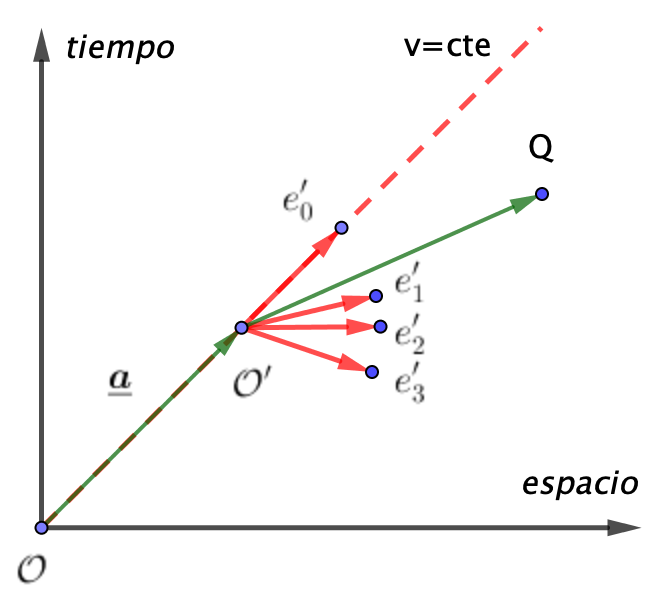
\includegraphics[width=.45\textwidth]{imagenes/img31-01.png}
\end{figure}


$Q=ct\ e_0+x\ e_1+y\ e_2+ z\ e_3 \ = $  

$=\ a^0e_0+a^1e_1+a^2e_2+a^3e^3+ \ $

$+\ ct'\ e'_0+x'\ e'_1+y'\ e'_2+ z'\ e'_3$

$\mqty(e'_0\\e'_1\\e'_2\\e'_3) \ = \ M \ \mqty(e_0\\e_1\\e_2\\e_3)$

$M$ matriz de cambio de base (aún desconocida).

\end{multicols}

$Q=\mqty(a^0 & a^1 & a^2 & a^3) \mqty(e_0 \\ e_1 \\ e_2 \\ e_3) +  \mqty(ct' & x' & y' & z') \mqty(e'_0 \\ e'_1 \\ e'_2 \\ e'_3)=$

$\mqty(a^0 & a^1 & a^2 & a^3) \mqty(e_0 \\ e_1 \\ e_2 \\ e_3)+ \mqty(ct' & x' & y' & z') \ M \mqty(e_0 \\ e_1 \\ e_2\\e_3)= \mqty(ct&x&y&z)\mqty(e_0 \\ e_1 \\ e_2 \\ e_3)$


$\left[ \mqty(a^0 & a^1 & a^2 & a^3)+ \mqty(ct' & x' & y' & z')\ M \right] \mqty(e_0 \\ e_1 \\ e_2\\e_3)= \mqty(ct&x&y&z)\mqty(e_0 \\ e_1 \\ e_2 \\ e_3)$

$\mqty(a^0 & a^1 & a^2 & a^3)+ \mqty(ct' & x' & y' & z')\ M\ = \ \mqty(ct&x&y&z)$

$\left[\  \mqty(ct' & x' & y' & z')\ M\  = \ \mqty(ct&x&y&z) \ - \   \mqty(a^0 & a^1 & a^2 & a^3) \ \right]^T$

$\textcolor{red}{({M^{-1})}^T} \ M^T \mqty(ct'\\x'\\y'\\z') \ = \ \textcolor{red}{({M^{-1})}^T} \ \mqty(ct-a^0\\x-a^1\\y-a^2\\z-a^3)$

Como en todos los libros de texto, llamamos $\ \boldsymbol{
\Lambda = (M^{-1})^T  }$


$ \boldsymbol{ \mqty(ct'\\x'\\y'\\z') \ = } \ \Lambda \ \mqty(ct-a^0\\x-a^1\\y-a^2\\z-a^3) \ = 
\ \boldsymbol{ \Lambda \ \left[ 
 \mqty(ct\\x\\y\\z-) -  \mqty(a^0\\a^1\\a^2\\a^3)
\right] }$


$\Lambda$ depende solamente de la velocidad relativa entre los observadores $\mathcal O$ y $\mathcal O'$, por lo que aplicada a la matriz $\underline a$ nos proporcionará una matriz constante que llamaremos $\Lambda \ \mqty(a^0\\a^1\\a^2\\a^3) = -\mqty(b^0\\b^1\\b^2\\b^3)$ y podremos escribir la transformación de coordenadas entre dos observadores inerciales como:


$\boldsymbol{ \mqty(ct'\\x'\\y'\\z') \ = \ \Lambda \ \mqty(ct\\x\\y\\z) \ + \ \mqty(b^0\\b^1\\b^2\\b^3) } \, , \ $ que usando el mismo truco del tema anterior,

$$\subrayado{\ \boldsymbol{
\mqty( ct'\\x'\\y'\\z'\\ \cdots \\ 1) \ = \ 
	\mqty(
		\boxed{\mqty{\\ &  &  \Lambda  & & \\ \\ \\}} &  \boxed{\mqty{b^0\\b^1\\b^2\\b^3}}
		\\ & \\
		\boxed{\mqty{\ 0&0&0&0 \ }} & \boxed{\mqty{1}}
	)
\ \mqty( ct\\x\\y\\z\\ \cdots \\ 1)
} \ }$$

Matriz que definirá lo que llamaremos \textbf{transformación de Poincaré} que tendrán estructura de Grupo multiplicativo de Lie. Nos queda aún por determinar la forma de las matrices $\Lambda$.

Para transformar lo que llamaremos \textbf{vectores Lorentz} usaremos solamente las matrices $\Lambda$ (que es como cambiar los $1$ por $0$ en las matrices primera y tercera de la ecuación anterior). Es decir, Llamaremos \emph{vector Lorentz} a cualquier cuaterna de número $(A^0, A^1, A^2, A^3)$ que al cambiar entre dos observadores inerciales se transformen así:

$$\subrayado{ \ \boldsymbol{
\mqty(A^{0'}\\A^{1'}\\A^{2'}\\A^{3'}) \ = \ \Lambda \ \mqty(A^0\\A^1\\A^2\\A^3)
} \ }$$


\vspace{5mm}
Vamos a determinar qué condiciones deben cumplir las matrices $\Lambda$:

$\lambda = (M^T)^{-1} \ \to \ M^T=\lambda^{-1} \ \to \ M=(\lambda^{-1})^T=(\lambda^T)^{-1}\, , \ $ inversa y traspuesta conmutan.

Tendremos que: $\qquad \mqty(e_{01}\\e_{1'}\\e_{2'}\\e_{3'})=(\Lambda^{-1})^T \mqty(e_0\\e_1\\e_2\\e_3)\ ; \ \ \ \qquad \mqty(A^{0'}\\A^{1'}\\A^{2'}\\A^{3'}) = \Lambda \mqty(A^0\\A^1\\A^2\\A^3)$

Son necesarias dos condiciones: que estemos tratando con \emph{tensores} (vectores) y que, para que los sistemas de referencia sea inerciales, la métrica tenga la misma forma $\ g'=g=\mqty(1\\ &-1\\ &&-1\\ &&&-1)$

El que estemos tratando con tensores significa que:

$\underline v=v^{0'}e_{0'}+v^{1'}e_{1'}+v^{2'}e_{2'}+v^{3'}e_{3'}=\mqty(v^{0'}&v^{1'}&v^{2'}&v^{3'})\mqty(e_{0'}\\e_{1'}\\e_{2'}\\e_{3'})=\mqty(v^{0'}&v^{1'}&v^{2'}&v^{3'}) (\Lambda^{-1})^T \mqty(e_0\\e_1\\e_2\\e_3)=$

$=\mqty(v^{0'}\\v^{1'}\\v^{2'}\\v^{3'})^T (\Lambda^{-1})^T \mqty(e_0\\e_1\\e_2\\e_3) = \left[ \Lambda \mqty(v^0\\v^1\\v^2\\v^3)\right]^T (\Lambda^{-1})^T \mqty(e_0\\e_1\\e_2\\e_3)=
\mqty(v^{0}&v^{1}&v^{2}&v^{3}) \ \Lambda \ 
(\Lambda^{-1})^T \ \mqty(e_0\\e_1\\e_2\\e_3)=$

$= \mqty(v^{0}&v^{1}&v^{2}&v^{3}) \ \mqty(e_0\\e_1\\e_2\\e_3)\, , \ $ relación que evidentemente se cumple al ser $\Lambda \ (\Lambda^{-1})^T=I$

Esto es lo que debe ocurrir para considerar a $\underline v$ un tensor (vector). Esto garantiza que estamos tratando con observadores.

Para exigir que estos observadores sean inerciales, necesitamos imponer también que $g=g'$, ambos han de calcular del mismo modo el producto escalar, $A'\cdot A'=A\cdot A \, . \ \ $
Vamos a usar que $A'=\Lambda A$ y que $\underline a \cdot \underline b = a^T\ g \ b$

$A'\cdot A'=(A')^T g (A')=(\Lambda A)^T g (\Lambda A)=A^T \Lambda^T g \Lambda A \ = \ A^T g A = A\cdot A $

Por lo que, necesariamente, $\quad \subrayado{ \ \boxed{\ \boldsymbol{ \Lambda^T \ g \ \Lambda \ = \ g  \ } } \ }$ y los observadores serán inerciales.

\vspace{5mm}
\begin{myblock}{Observadores inerciales}

\vspace{3mm} Estaremos hablando de observadores si 

\begin{equation}
\label{T31Observadores}
A' \ = \ \Lambda \ A \qquad \text { y } \qquad
 e'\ = \ {(\Lambda^{-1})}^T \ e
\end{equation}
 
 y serán inerciales si
 
 \begin{equation}
 \label{T31Inerciales}	
 \Lambda^T \ g \ \Lambda \ = \ g
 \end{equation}

\end{myblock}

\vspace{1cm}

\begin{example}

En el capítulo anterior, para el caso de un espacio-tiempo de 1+1 dimensiones espaciales y temporales, obtuvimos  $\ \Lambda=\mqty(\gamma&-\gamma \beta \\-\gamma\beta & \gamma)$, con $\gamma=\dfrac 1 {\sqrt{1-\beta^2}}$ siendo $\beta =\dfrac v c$. Veamos como esta matriz sí cumple la condición de observadores inerciales, ec. \ref{T31Inerciales}:

\vspace{5mm}
$\Lambda^T g \Lambda=
\mqty(\gamma&-\gamma \beta \\-\gamma\beta & \gamma) \mqty(1&0\\0&-1)\mqty(\gamma&-\gamma \beta \\-\gamma\beta & \gamma)=$

$=\mqty(\gamma&-\gamma \beta \\-\gamma\beta & \gamma)\mqty(\gamma&-\gamma \beta \\ \gamma\beta & -\gamma)=
\gamma^2 \mqty(1&-\beta \\ -\beta&1) \mqty(1&-\beta\\\beta&-1)=\gamma^2 \mqty(1-\beta^2&0\\0&\beta^2-1)=$

$=\cancelto{1}{\gamma^2 (1-\beta^2)}\mqty(1&0\\0&-1)=g\, , \ $ efectivamente, $\ \Lambda^T g \Lambda=g$
	
\end{example}


\vspace{1cm} Para cualquier transformación de coordenadas, sean rotaciones o boosts, se usarán los \emph{generadores de Lorentz}\footnote{ Ver capítulo 15, ``El grupo de Poincaré 1/3'' del curso de ``Grupos de Lie'' de \emph{Javier García}. \\ Apunte en \textcolor{blue}{https:\\igvaori.github.io}}. Presentamos una versión reducida:

$\Lambda = e^{matriz} \, , \ \text{ con } \ matriz=aK^1+bK^2+cK^3+n_1J^1+n_2J^2+n_3J^3$, siendo $K^1,K^2,K^3$ los generadores del boost en los ejes $x,y,z$ y $J^1,J^2,J^3$ las matrices generadoras de las rotaciones en los ejes $x,y,z$ respectivamente.




$$K^1=\begin{pmatrix} 0 & 1 & 0 & 0 \\ 1 & 0 & 0 & 0 \\ 0 & 0 & 0 & 0 \\ 0 & 0 & 0 & 0 \end{pmatrix};\quad K^2=\begin{pmatrix} 0 & 0 & 1 & 0 \\ 0 & 0 & 0 & 0 \\ 1 & 0 & 0 & 0 \\ 0 & 0 & 0 & 0 \end{pmatrix};\quad K^3= \begin{pmatrix} 0 & 0 & 0 & 1 \\ 0 & 0 & 0 & 0 \\ 0 & 0 & 0 & 0 \\ 1 & 0 & 0 & 0 \end{pmatrix}$$ 

$$J^1=\begin{pmatrix} 0 & 0 & 0 & 0 \\ 0 & 0 & 0 & 0 \\ 0 & 0 & 0 & -1 \\ 0 & 0 & 1 & 0 \end{pmatrix};\quad J^2=\begin{pmatrix} 0 & 0 & 0 & 0 \\ 0 & 0 & 0 & 1 \\ 0 & 0 & 0 & 0 \\ 0 & -1 & 0 & 0 \end{pmatrix};\quad J^3=\begin{pmatrix} 0 & 0 & 0 & 0 \\ 0 & 0 & -1 & 0 \\ 0 & 1 & 0 & 0 \\ 0 & 0 & 0 & 0 \end{pmatrix} $$

\vspace{5mm}

\hspace{1cm} $\boldsymbol{ 
\Lambda =exp\left[ a\begin{pmatrix} 0 & 1 & 0 & 0 \\ 1 & 0 & 0 & 0 \\ 0 & 0 & 0 & 0 \\ 0 & 0 & 0 & 0 \end{pmatrix}+b\begin{pmatrix} 0 & 0 & 1 & 0 \\ 0 & 0 & 0 & 0 \\ 1 & 0 & 0 & 0 \\ 0 & 0 & 0 & 0 \end{pmatrix}+c\begin{pmatrix} 0 & 0 & 0 & 1 \\ 0 & 0 & 0 & 0 \\ 0 & 0 & 0 & 0 \\ 1 & 0 & 0 & 0 \end{pmatrix}+  \right. } $

$\boldsymbol{ \qquad \qquad \qquad \qquad  \left.  +n_{ 1 }\begin{pmatrix} 0 & 0 & 0 & 0 \\ 0 & 0 & 0 & 0 \\ 0 & 0 & 0 & -1 \\ 0 & 0 & 1 & 0 \end{pmatrix}+n_{ 2 }\begin{pmatrix} 0 & 0 & 0 & 0 \\ 0 & 0 & 0 & 1 \\ 0 & 0 & 0 & 0 \\ 0 & -1 & 0 & 0 \end{pmatrix}+n_{ 3 }\begin{pmatrix} 0 & 0 & 0 & 0 \\ 0 & 0 & -1 & 0 \\ 0 & 1 & 0 & 0 \\ 0 & 0 & 0 & 0 \end{pmatrix} \right] }$


\vspace{5mm}

\underline{Ejemplo: boost dirección $x$} $\quad \Lambda=e^{\theta K^1}$

Por Taylor, $e^M=I+M+\dfrac 1 2 M^2 + \dfrac 1 {3!} M^3 + \cdots$,

$\Lambda=e^{\theta K^1}=I+(\theta K^1) + \dfrac 1 2 \theta^2 (K^1)^2 + \dfrac 1{3!} \theta^3 (K^1)^3 + \cdots $

Como $\ (K^1)^2= \mqty(1&0&0&0\\0&1&0&0 \\0&0&0&0\\0&0&0&0)=\mqty(I_2&0\\0&0) \ $ y $\ (K^1)^3=K^1=\mqty(0&1&0&0\\1&0&0&0\\0&0&0&0\\0&0&0&0)\, , \ $ tenemos 

$A=I+\theta K^1+\dfrac 1 2 \theta^2 \mqty(I_2&0\\0&0)+ \dfrac 1{3!} \theta^3 K^1 + \cdots = I+\left( \theta + \dfrac 1{3!} \theta^3 + \dfrac 1 {5!} \theta^5 + \cdots \right)  K^1 + \left( \dfrac 1{2!} \theta^2 + \dfrac 1{4!} \theta^4 + \cdots \right) \mqty(I_2&0\\0&0) =$

$=I+\sinh \theta K^1 + (\cosh \theta - 1 ) \mqty(I_2&0\\0&0)$

$\Lambda=e^{\theta K^1}= \mqty(I_2&0\\0&I_2) + \mqty(0 & \\sinh \theta &0&0\\ \sinh \theta &0&0&0 \\ 0&0&0&0 \\ 0&0&0&0 ) + \mqty(\cosh \theta -1 &0&0&0 \\ 0&\cosh \theta - 1 &0&0 \\ 0&0&0&0 \\ 0&0&0&) =$

$=\mqty( \cosh \theta & \sinh \theta &0&0\\ \sinh \theta & \cosh \theta &0&0\\ 0&0&1&0\\0&0&0&1) = \Lambda(\theta)\quad $
Para $\ \Lambda(-\theta) \ = \ \mqty( \cosh \theta & -\sinh \theta &0&0\\ -\sinh \theta & \cosh \theta &0&0\\ 0&0&1&0\\0&0&0&1) \ $ que es la transformación que obtuvimos para pasar $\ \mqty(ct'\\x')=\Lambda \mqty(ct\\x)$

Si hubiésemos hecho $\ \Lambda=e^-\theta K^2=\mqty( \cosh \theta &0&-\sinh \theta & 0 \\ 0&1&0&0 \\ -\sinh \theta&0&\cosh \theta &0 \\ 0&0&0&1)$

Para una rotación en torno al eje $z$, $\quad \Lambda=e^{\theta J^3} = \mqty(1 & \mqty{0&0&0}\\ \mqty{0\\0\\0} & R_z)=	\mqty( 1&0&0&0\\ 0&\cos \theta & -\sin \theta & 0 \\ 0& \sin \theta & \cos \theta & 0 \\ 0&0&0&1)$


En general, $\ \Lambda=e^{aK^1+bK^2+cK^3+n_1J^1+n_2J^2+n_3J^3}\ $ que es la matriz de transformación general o boost generalizado entre dos observadores inerciales.

\vspace{5mm} Ha de ocurrir $\ det(\Lambda)=1\ $.

Evidentemente, como $\Lambda^T g \ \Lambda =g\  \to \  \det(\Lambda^T g \ \Lambda)= (\det(\Lambda))^2 det(g)=\det (g) \ \to \  (\det(\Lambda))^2 =1 \ \to \ $ tomamos $\ \det \Lambda =1$ ya que si $\det \Lambda=-1 \ \to \ \Lambda \neq I $ y no podemos reproducir el hecho que ambos observadores sean el mismo, $\mathcal O=\mathcal O'$ y $a=b=c=n_1=n_2=n_3=0$ con lo que $\Lambda = e^{0+0+0+0+0+0}=e^0 = I$

De otro modo, como $det(e^M)=e^{traza\ M}$ y $traza(M+N)=traza(M)+traza(N)$,  como además se cumple que 
$traza(K^i)=traza(J^j)=0$, entonces, 
$\det \Lambda=\det e^M=e^{0+0+0+0+0+0}=e^0=1$

\begin{myalertblock}{Grupo de Lorentz $SO(1,3)$}

\begin{equation}
\label{T31GL}
\boldsymbol{
	SO(1,3) \ = \	\{ \ \Lambda \ / \ det \Lambda \ = \  1 \quad \wedge \quad \Lambda^T g \ \Lambda \ = \ g  \ \}
}
\end{equation}

\begin{center} \vspace{5mm}con $\quad g=\mqty(1\\&-1\\&&-1\\&&&-1)$ \end{center}
\end{myalertblock}

Para que nuestra teoría cumpla con los requisitos de la relatividad especial ha de ser invariante bajo transformaciones del grupo $SO(1,3)$ de Lorentz.

Las rotaciones, $SO(3)=\{R \ / \ RR^T=I \ \ \wedge  \ \ det R=1 \}$ están incluidas en el grupo de Lorentz, $\ SO(3) \subset SO(1,3) \ $

Si incluimos las traslaciones espacio-temporales en el grupo de Lorentz, tenemos el \textbf{grupo de Poincaré}

\begin{myalertblock}{Grupo de Poincaré}

\begin{equation}
\label{T31GP}
\boldsymbol{
	\mqty( 
		\boxed{\mqty{\\\Lambda \in SO(1,3)\\ \\ } } & \boxed{\mqty{a^0\\a^1\\a^2\\a^3}} 
		\\ 
		\boxed{ \mqty{0&0&0&0} }& \boxed{1} 
	) 
}	
\end{equation}
	
\end{myalertblock}


\vspace{5mm} En una teoría de campos en la que no existan puntos ni  direcciones especiales, $\mathcal L=\neq \mathcal L(ct,x,y,z)$ sino que $\mathcal L = \mathcal L(\phi, \partial_\mu \phi)$, este tipo de langrangianos también deben ser invariantes bajo transformaciones del grupo de Poincaré.







